% !TEX encoding = UTF-8 Unicode
\documentclass[11pt, a4paper]{article}
\usepackage{authblk}
\linespread{1.2}
\usepackage{palatino}
\usepackage{parskip}
\usepackage{graphicx}
\usepackage[colorlinks,linktocpage]{hyperref}
\usepackage[listings]{tcolorbox}

% Title
\title{Manual for tsRFinder}
\author{Qinhu Wang}
\author{Weixing Shan\thanks{Email: wxshan@nwafu.edu.cn}}
\affil{Northwest A\&F University}
\date{Version 1.0.0\\[3pt] \today}

%%% Begin document
\begin{document}

\maketitle

\begin{abstract}
The tsRFinder is a lightweight, fast and reliable tool for prediction and annotation of tRNA-derived small RNAs using next-generation sequencing data. It's a free open source software available at \url{https://github.com/wangqinhu/tsRFinder}.
\end{abstract}

\clearpage

\tableofcontents

\clearpage

\section{Introduction}

Small RNAs, such as miRNA, siRNA, and piRNA, are key regulators of gene expression. The tRNA-derived small RNA (tsRNA) is a recently identified novel class of small RNA, no public tool has tailored for tsRNA analysis yet. We thus developed tsRFinder for tsRNA prediction and annotation with additional sequence and statistical analysis, using small RNA sequencing data and the reference genome sequences.

\section{How to install}

\subsection{Dependency}

The tsRFinder depends on a few free open source softwares, please check and install them at first:

\begin{itemize}

\item Perl, v5.10.1 or higher, required for tsRFinder.pl execution. Always build-in in most of the UNIX-like OS. \\\url{http://www.perl.org/get.html}
\item R, v2.15.2 or higher, required for small RNA data analysis and illustration. \\\url{http://www.r-project.org}
\item bowtie, v1.0.0 or higher, required for small RNA mapping. \\\url{https://github.com/BenLangmead/bowtie}
\item tRNAscan-SE, v1.3.1 or higher, required for tRNA prediction. It's optional if you prefer manual tRNA input. \\\url{http://lowelab.ucsc.edu/tRNAscan-SE}

\end{itemize}

\subsection{Installation}

tsRFinder is maintained on GitHub and is ready-to-use, no compilation is required. However, if you take some time to improve the configuration, it may save you a lot of time for trouble shooting.

First, you may clone \footnote{If git is not installed, download it from \url{http://git-scm.com}} tsRFinder by typing the following in the terminal.

{\footnotesize \begin{tcolorbox}[colback=blue!5!white,colframe=blue!75!black,title=Clone tsRFinder]
\begin{verbatim}
git clone https://github.com/wangqinhu/tsRFinder.git
\end{verbatim}
\end{tcolorbox}}

Alternatively, you may download it from the following URL.

{\footnotesize \begin{tcolorbox}[colback=blue!5!white,colframe=blue!75!black,title=Latest release of tsRFinder]
\begin{verbatim}
https://github.com/wangqinhu/tsRFinder/releases/latest
\end{verbatim}
\end{tcolorbox}}

Once tsRFinder is cloned or unpacked, move the entire directory to a proper place (or current working directory, such as home directory) and add the tsRFinder path to your environment settings. For example, if tsRFinder is placed in /the/path/of/tsRFinder, then type the following in the terminal if you are using bash.


{\footnotesize \begin{tcolorbox}[colback=blue!5!white,colframe=blue!75!black,title=Setup tsRFinder]
\begin{verbatim}
echo export tsR_dir="/the/path/of/tsRFinder" >> $HOME/.bashrc
source ~/.bashrc
\end{verbatim}
\end{tcolorbox}}

tsRFinder is now ready for your dataset.

\section{How to use}

\subsection{Preparing the dataset}

Before running tsRFinder, you are asked to prepare/download the following two files: (1) the reference genome sequence, or the reference tRNA sequence and, (2) the small RNA reads.

You are strongly recommended to use the reference genome sequence and raw small RNA sequencing data since tsRFinder is capable of preparing the reference tRNA data and clean small RNA data automatically. In case you prefer to preparing tRNA and small RNA files manually, see "demo/tRNA.fas" and "demo/sRNA.fa.gz" or access the format description in the FAQ section.

\subsection{Running the pipeline}

tsRFinder has two ways for arguments input, either configuration file or command line option. We recommend you to use a command line option for debugging and building your configuration file. Once your inputs are determined, you can write it to a configuration file for analysis.

Once tsRFinder is properly installed, you can run tsRFinder from terminal directly, see the usage below.

{\scriptsize \begin{tcolorbox}[colback=blue!5!white,colframe=blue!75!black,title=Usage of tsRFinder: ./tsRFinder.pl -h]
\begin{verbatim}

tsRFinder usage:

    tsRFinder.pl <option>

    -c  Configuration file
    -l  Label
    -g  Reference genomic sequence file, conflict with -t
    -t  Reference tRNA sequence file, conflict with -g
    -s  Small RNA sequence file
    -a  Adaptor sequence
    -n  Min read length            [default 18]
    -x  Max read length            [default 45]
    -e  Min expression level       [default 10]
    -u  Mature tsRNA level cut-off [default 10]
    -f  Small RNA family threshold [default 72]
    -w  tRNA with/without label    [default no/yes]
    -o  Output compressed tarball  [default no/yes]
    -m  Mode, run/debug            [default run/debug]
    -h  Help
    -v  Version

Examples:

    tsRFinder.pl -c demo/tsR.conf

    tsRFinder.pl -c demo/tsR.alt.conf
\end{verbatim}
\end{tcolorbox}}


\section{Demo}

To have a quick but rough overview that how tsRFinder looks like, see the animated gif demo in doc/demo.gif or online.

\subsection{Demo data}

\textbf{Demo refseq}: we used several random sequences embedded with some real tRNAs as pseudo reference sequences, in FASTA format and accessible from file "tsRFinder/demo/genome.fa". A reference genome sequence is also applicable. Figure \ref{refseq} shows a refseq file in FASTA format.

\begin{figure}[htbp]
\begin{center}
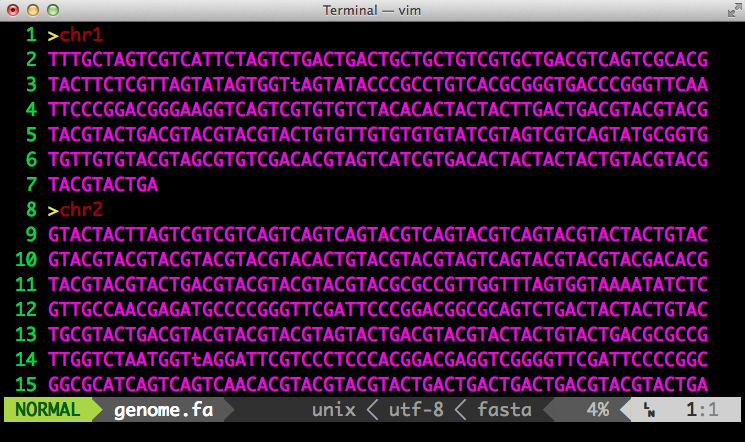
\includegraphics[width=12cm]{refseq.png}
\caption{Screenshot of the reference sequence in FASTA format} 
\label{refseq}
\end{center}
\end{figure}

\textbf{Demo sRNA}: we extracted a bit of raw reads from some experimental data as a demo. Each read of the raw small RNA data have 4 lines. Beginning with "@" identifier line, followed by sequence line, "+" identifier optional line and quality score line, as shown in Figure \ref{fastq}.

\begin{figure}[htbp]
\begin{center}
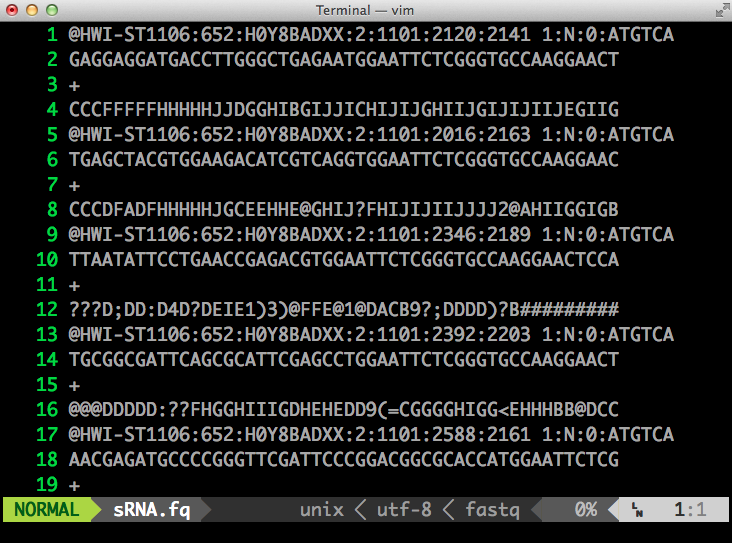
\includegraphics[width=12cm]{fastq.png}
\caption{Screenshot of the small RNA sequence in FASTQ format} 
\label{fastq}
\end{center}
\end{figure}

\subsection{Demo running}

tsRFinder allows you specify inputs via a separate configuration file, as shown below for an example of the content of demo tsR.conf:

{\footnotesize \begin{tcolorbox}[colback=blue!5!white,colframe=blue!75!black,title=Demo configuration file for tsRFinder: demo/tsR.conf]
\begin{verbatim}

label               :  Abc
reference_genome    :  demo/genome.fa
reference_tRNA      :
sRNA                :  demo/sRNA.fq.gz
adaptor             :  TGGAATTCTCGGGTGCCAAGG
min_read_length     :  18
max_read_length     :  45
min_expression_level:  10
mature_cut_off      :  10
family_threshold    :  72
tRNA_with_label     :  no
output_compressed   :  no

\end{verbatim}
\end{tcolorbox}}

Currently we have 12 items (16 options in command line) for configuration file filling. The argument items and the inputs are separated by colon (":"). You are recommended to use the first three letters of the investigated organism as a label (e.g. Ath for \textit{Arabidopsis thaliana}, \emph{-l} in command line option); the paths of reference genome (\emph{-g}) and small RNA (\emph{-s}) should be supplied at least (tsRFinder supports input in gzipped files for sRNA and reference genome, and plain ASCII text is also acceptable). If raw sequence data is used, the adaptor sequence (\emph{-a}) is required. In case a reference tRNA (\emph{-t}) is not used, leave the argument to EMPTY.

Once the configuration file (-c) is prepared, an analysis protocol have been determined. In the demo, the configuration file is at demo/tsR.conf, typing the following in the terminal to run tsRFinder:

{\footnotesize \begin{tcolorbox}[colback=blue!5!white,colframe=blue!75!black,title=Running tsRFinder demo]
\begin{verbatim}
./tsRFinder.pl -c demo/tsR.conf
\end{verbatim}
\end{tcolorbox}}

To run alternative tRNA and sRNA dataset prepared yourself, typing the following:

{\footnotesize \begin{tcolorbox}[colback=blue!5!white,colframe=blue!75!black,title=Running tsRFinder alternative demo]
\begin{verbatim}
./tsRFinder.pl -c demo/tsR.alt.conf
\end{verbatim}
\end{tcolorbox}}

tsRFinder allows you specify the minimum (\emph{-n}) and maximum (\emph{-x}) length of sequence for processing, you may specify the minimum expression level (\emph{-e}) of the reads to increase reliability, as well as cut-off (\emph{-u}) of the expression level of mature tsRNA. In case the family members are loose, the users may increase the tsRNA family threshold (\emph{-f}) to tune it.

tsRFinder can work in run and debug modes (\emph{-m}). In case of accessing some problems or some temporary files, you may enable the debug mode, otherwise use the run mode (default). To check the usage or version, you can use \emph{-h} and \emph{-v} option, respectively. To create a compressed tarball of the output file, use \emph{-o yes} option please.

\subsection{Demo output}

By default, tsRFinder delivers a summary files with some basic statistics. The predicted or user applied tRNA sequence, the small RNA clean data, the tRNA reads, and the predicted tsRNA sequences are listed. A figure showing the length distributions of small RNA and tRNA reads (Figure \ref{distribution}) are included. Meanwhile, tsRFinder gives additional summary on tsRNA family, and tRNA/tsRNA expression levels (including 5' tsRNA, 3' tsRNA and their abundance), text map (tmap) showing mapping of small RNA to tRNA, graphics showing the expression level based on small RNA data, the cleavage sites, and the cleavage profile (Figure \ref{cleavage}).
Shown below is a demo:

{\footnotesize \begin{tcolorbox}[colback=blue!5!white,colframe=blue!75!black,title=tsRFinder demo output list]
\begin{verbatim}

---------
 SUMMARY 
---------

*     tRNA seq : Abc/tRNA.fa
         Total : 5
*   sRNA reads : Abc/sRNA.fa
         Total : 10005215
        Unique : 7227
*   tRNA reads : Abc/tRNA.read.fa
         Total : 236122
        Unique : 50
*    tsRNA seq : Abc/tsRNA.seq
         Total : 7
        Unique : 6
* tsRNA report : Abc/tsRNA.report.xls
  tsR-5p total : 5
  tsR-3p total : 2
 tsR-5p unique : 4
 tsR-3p unique : 2
*     Text map : Abc/tsRNA.tmap
*   Visual map : Abc/images
* Distribution : Abc/distribution.pdf
*     Cleavage :
        Detail : Abc/cleavage.txt
       Profile : Abc/cleavage_profile.pdf
* tsRNA family : Abc/tsRNA.fam
* Stat. by BDI :
   Sensitivity : 0.9593
   Specificity : 0.7825
      Accuracy : 0.8819

\end{verbatim}
\end{tcolorbox}}

\begin{figure}[htbp]
\begin{center}
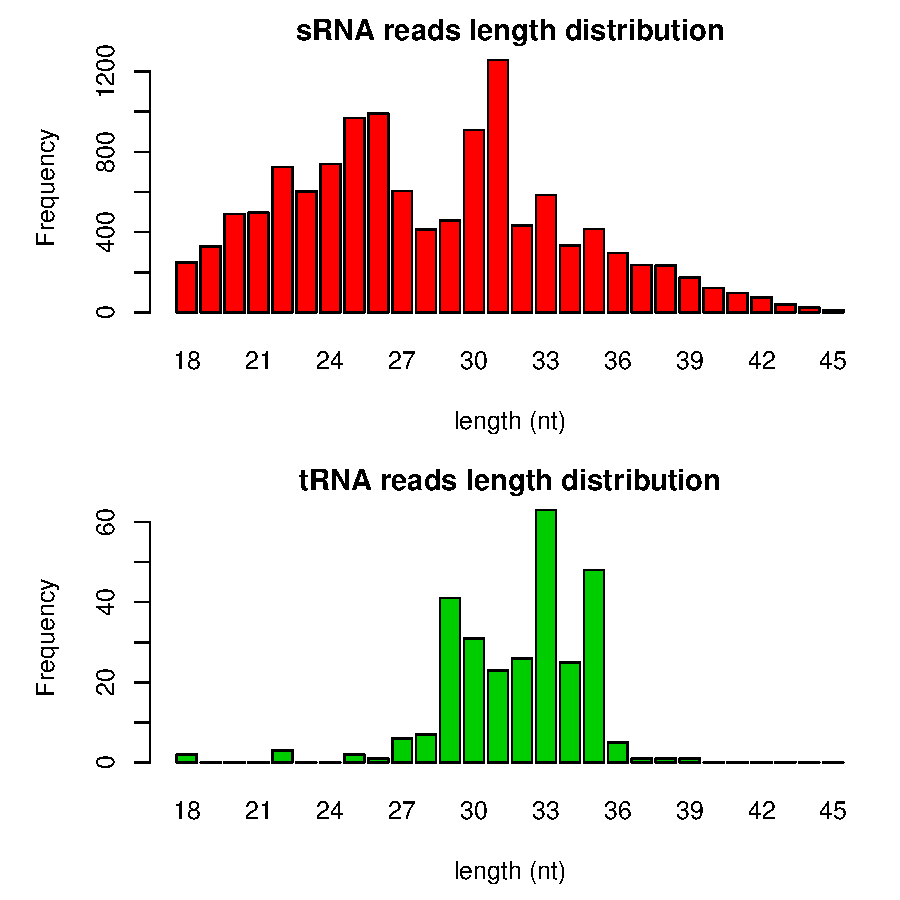
\includegraphics[width=12cm]{distribution.pdf}
\caption{Length distribution of small RNA and tRNA reads}
\label{distribution}
\end{center}
\emph{Note:} The range of the small RNA length exhibited here is based on the minimum (\emph{-n}) and maximum (\emph{-x}) sequence length that specified in command line or the configuration file.
\end{figure}

\begin{figure}[htbp]
\begin{center}
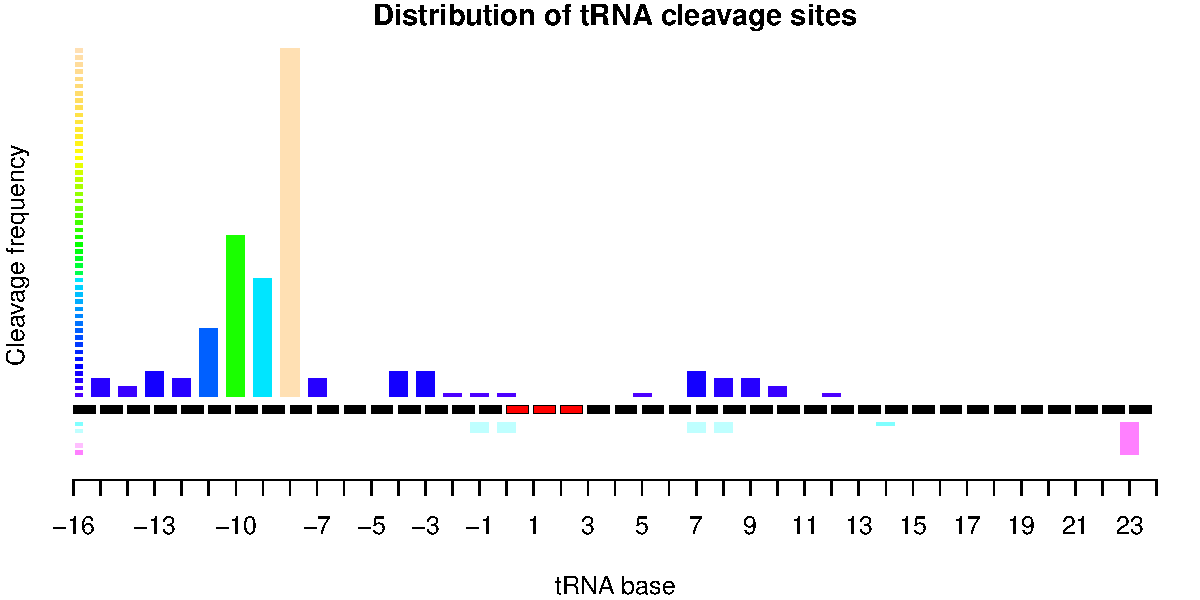
\includegraphics[width=13cm]{cleavage_profile.pdf}
\caption{tRNA cleavage profile}
\label{cleavage}
\end{center}
\emph{Note:} This figure is based on TAIR10 and \textit{Arabidopsis thaliana} small RNA data GSM154336. The demo data contains only a few reads with limited cleavage information was not shown.
\end{figure}

\subsection{Visualization of tmap data}

To examine the map of tsRNA, a vim syntax plugin was developed for visualization. You may enable color text map by copying lib/tmap.vim into the vim syntax folder, and put the following line into your .vimrc file:

{\footnotesize \begin{tcolorbox}[colback=blue!5!white,colframe=blue!75!black,title=Set filetype tmap in vim]
\begin{verbatim}
au BufNewFile,BufRead *.tmap setf tmap
\end{verbatim}
\end{tcolorbox}}

Once tmap vim is installed, open the tsRNA.tmap file with vim to generate a color text map, as shown in Figure \ref{tmap}.

{\footnotesize \begin{tcolorbox}[colback=blue!5!white,colframe=blue!75!black,title=Visualization tsRNA.tmap]
\begin{verbatim}
vim tsRNA.tmap
\end{verbatim}
\end{tcolorbox}}

\begin{figure}[htbp]
\begin{center}
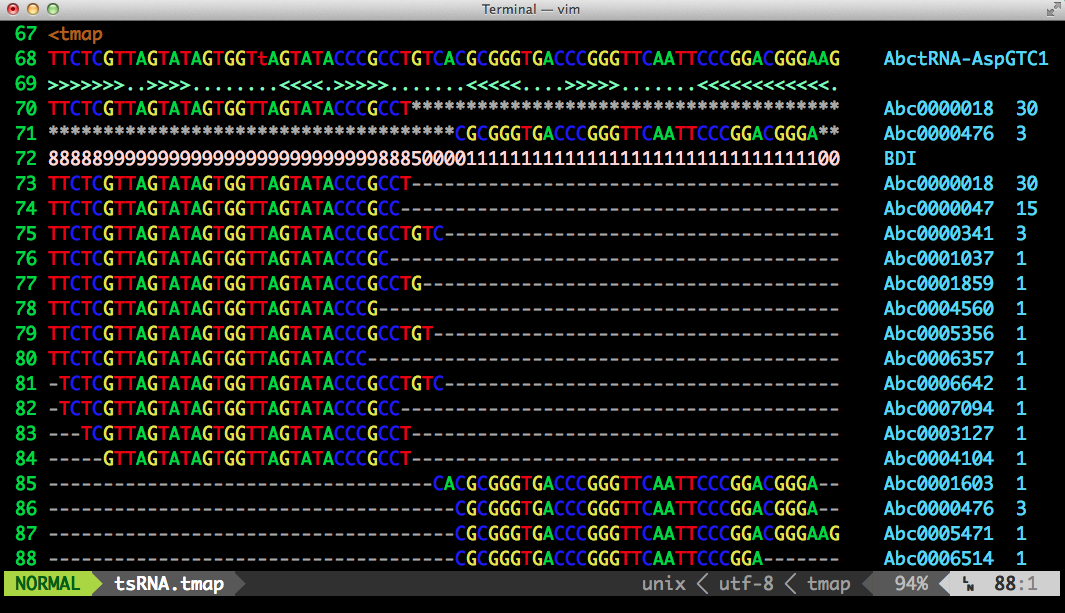
\includegraphics[width=12cm]{tmap.png}
\caption{Screenshot of color tmap} 
\label{tmap}
\end{center}
\end{figure}

If you prefer plain text view without highlighting, open tsRNA.tmap with any text editors you have.

\section{FAQ}

\textbf{1. Can tsRFinder run on Windows?}

No. tsRFinder depends on tRNAscan-SE (UNIX source code) and uses the advantages of some build-in program of UNIX-like systems, for example, awk, grep and head. Running on Windows may lead unexpected errors. Linux or OS X is strongly recommended.

\textbf{2. What's the length required for small RNA reads?}

Ideally, sequences from 15 - 50 nt for small RNA are recommend.

\textbf{3. What's the tRNA format required for input?}

You are encouraged to use reference genomic sequences since tsRFinder is capable of extracting tRNA sequences via tRNAscan-SE, removing duplicated sequences, and formatting the input. In case a manually prepared file is preferred, proceed following this format: first line, begin with "$>$", followed by label "$Abc$", and the name of tRNA "$tRNA-ProCGG1$"; second line, the sequence of tRNA; and third line, the secondary structure of tRNA, "$><$" and "$()$" both are acceptable. Be carefully in preparing this because "$>$" equals "$($" but not "$)$".\\
Shown below is an example.

{\scriptsize \begin{tcolorbox}[colback=blue!5!white,colframe=blue!75!black,title=tRNA example]
\begin{verbatim}
>AbctRNA-ProCGG1
GGCCTCGTGGTCTAGTGGTATGATTCTC [NNN] AGAGGtCCCGGGTTCGATTCCCGGTGAGGCCC
>>>>>>>..>>>.........<<<.>>> [<.>] <<.....>>>>>.......<<<<<<<<<<<<.
\end{verbatim}
\end{tcolorbox}}

\textbf{4. What's the sRNA format required for input?}

You are recommended to use raw data. In case a manually prepared sRNA file is used for input, proceed following this format: first line, begin with "$>$", and the label "$Abc$", then the 7\-bit index, followed by "$\_$" (or "$|$", "$-$" and white space) and the read number; second line, the sequence of the read. One more thing, the format of sRNA data in tsRFinder is compatible with the FASTX\_TOOL kit \footnote{\url{http://hannonlab.cshl.edu/fastx_toolkit/}}, which helps you on processing the raw sequencing data.\\
Shown below is an example.

{\scriptsize \begin{tcolorbox}[colback=blue!5!white,colframe=blue!75!black,title=sRNA example]
\begin{verbatim}
>Abc0000001_772
CAGGTGGTCAGGTAGAGAATACCAAGGCGCT
>Abc0000002_475
AGGTGGTCAGGTAGAGAATACCAAGGCGCT
\end{verbatim}
\end{tcolorbox}}


\textbf{5. I have problems in installing tsRFinder and/or the dependencies, where can I get more help?}

You can access the official support website for trouble-shooting, or open new issue for tsRFinder repository on GitHub. The URL is \url{https://github.com/wangqinhu/tsRFinder/issues/new}

\textbf{6. Where to report bugs?}

Goto \url{https://github.com/wangqinhu/tsRFinder/issues/new}

\textbf{7. Can we use tsRFinder for commercial purpose?}

Yes. tsRFinder is free, open source software, see the MIT license.

\textbf{8. The 'nwalign' not compatible to my operating system, what can I do?}
 
tsRFinder uses Needleman-Wunsch algorithm nwalign for small RNA alignment, with pre-building of the binaries for some of the recent OS X / Linux. If you find it not suitable for your system or want to compile it by yourself, goto lib/src directory and type 'make' to build \footnote{The gcc compiler is required. For OS X, you can install Xcode (ship with gcc)} it manually.

\end{document}
